% 依据固定来源 PDF 第 1 页重绘；source_id=src-3612a22ce3848ad6ebbec4d94861dd64b009980e14e8c7a83efefb2ea39bd367
% PDF SHA-256: 2cea664b02860c04aa21fb6bdf80403b674befb8e61fa9f68970197bdf0f5ff4
\begin{center}
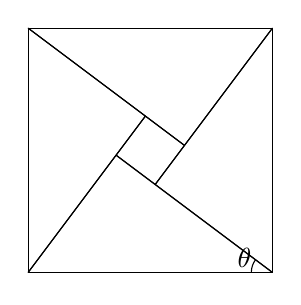
\begin{tikzpicture}[scale=0.62,line join=round,line cap=round]
  \coordinate (A) at (0,0);
  \coordinate (B) at (5,0);
  \coordinate (C) at (5,5);
  \coordinate (D) at (0,5);
  \coordinate (P) at (1.8,2.4);
  \coordinate (Q) at (2.6,1.8);
  \coordinate (R) at (3.2,2.6);
  \coordinate (S) at (2.4,3.2);
  \draw (A)--(B)--(C)--(D)--cycle;
  \draw (A)--(P)--(B);
  \draw (B)--(Q)--(C);
  \draw (C)--(R)--(D);
  \draw (D)--(S)--(A);
  \draw (P)--(Q)--(R)--(S)--cycle;
  \draw (4.57,0) arc[start angle=180,end angle=143.13,radius=0.43];
  \node at (4.43,0.30) {$\theta$};
\end{tikzpicture}
\end{center}
